\section{Differentiability}

You are likely familiar with differentiability (and particularly the computation of derivatives) from calculus. While this knowledge should certainly not be disregarded, we are going to go from the beginning, doing everything with a little more care than it got in calculus.
Throughout this section we will deal with functions $f: A \subseteq \R \rightarrow \R$,
though the basic definitions will apply to $\C$.\footnote{We will use differentiation over $\C$ in our discussion of power series though. One should also note that the other basic rules such as the sum, product and chain rules will also hold over $\C$, but being differentiable over $\C$ is a stronger condition than being differentiable over $\R$ or $\R^2$. For example, consider $f(z) = \overline{z}$, which is not complex differentiable.}.

Here's our basic definition:

\begin{definition}[Differentiability]
	Let $A \subseteq \R$ and $f: A \rightarrow \R$. 
	Then if $x$ is a limit point of $A$, we say that $f$ is \vocab{differentiable at $x$} with derivative $f'(x)$ if
	$$
	\lim_{h \to 0} \frac{f(x + h) - f(x)}{h} = f'(x).
	$$

	We say that $f$ is \vocab{differentiable} on $A$ if $f$ is differentiable at every $x \in A$.
\end{definition}

Let's pause for a moment. The core idea of differentiation is 
we want to \emph{approximate a function around some point using a linear map}\footnote{Indeed it is which this idea, not really that of `the tangent to a curve' that is used to generalise the derivative to functions of multiple variables. Of course they are closely related.}. Indeed, our definition of the derivative is directly equivalent to the following: $f$ is differentiable at $x$ if
$$
	f(x + h) = f(x) + f'(x)h + \varepsilon(h),
$$
where $\lim_{h\to 0} \varepsilon(h)/h = 0$. That is, it is differentiable if we can approximate the function with some linear map where the error decreases faster than linearly.


% \begin{remark}[Notation]
% 	It is common to write $f'(x) = \frac{\mathrm{d} y}{\mathrm{d} x} = \frac{\mathrm{d} f}{\mathrm{d} x}$, all of which work equally well.
% \end{remark}

\subsection{Properties of Differentiable Functions}

With that spiel over, we can move on to some properties of differentiable functions. The first is that differentiability implies continuity.

\begin{proposition}[Differentiability Implies Continuity]
	If $f$ is differentiable at $x$, then $f$ is continuous at $x$.
\end{proposition}
\begin{proof}
	Using the limit definition of continuity we have
	$$\lim_{h \to 0} \left[f(x + h) - f(x)\right] = \lim_{h \to 0} \frac{f(x + h) - f(x)}{h} \cdot (h) = f'(x) \cdot 0 = 0,
	$$
	thus $\lim_{h \to 0} f(x + h) = f(x)$, so $f$ is continuous at $x$.
\end{proof}

Now we can prove some basic rules for computing derivatives.

\begin{proposition}[Sum, Produt \& Quotient Rules]
	Suppose that $f: \R \rightarrow \R$ and $g: \R \rightarrow \R$ are differentiable at $x$ with derivatives $f'(x)$ and $g'(x)$.
	Then the following hold.
	\begin{enumerate}[label=(\roman*)]
		\item $f + g$ is differentiable at $x$, with $(f + g)'(x)= f'(x) + g'(x)$,
		\item $fg$ is differentiable at $x$, with $(fg)'(x) = f'(x)g(x) + f(x)g'(x)$,
		\item If $g'(x) \neq 0$ then $f/g$ is differentiable at $x$, with $(f/g)'(x) = \frac{g(x)f'(x) - g'(x)f(x)}{g^2(x)}$.
	\end{enumerate}
\end{proposition}
\begin{proof}
	We prove each individually.
	\begin{enumerate}[label=(\roman*)]
		\item This follows from the sum of limits.
		\item We have by the continuity of $f$
		\begin{align*}
			&\lim_{h \to 0} \frac{f(x + h)g(x + h) - f(x)g(x)}{h} \\
			=\ &\lim_{h \to 0}\left[ f(x+h) \frac{g(x + h) - g(x)}{h} + g(x)\frac{f(x + h) - f(x)}{h}\right],
		\end{align*}
		and by the continuity of $f$ and $g$ at $x$ we have $(fg)'(x) = f(x)g'(x) + f'(x) g(x)$.
		\item Similarly we have
		\begin{align*}
			&\lim_{h \to 0} \frac{f(x + h)/g(x + h) - f(x)/g(x)}{h} \\
		=\ &\lim_{h \to 0} \frac{1}{g(x)g(x + h)} \left[g(x)\frac{f(x + h) - f(x)}{h} - f(x) \frac{g(x + h) - g(x)}{h}\right],
		\end{align*}
		and by the continuity of $f$ and $g$ we have $(f/g)'(x) = \frac{g(x)f'(x) - g'(x)f(x)}{g^2(x)}$. \qedhere
	\end{enumerate}
\end{proof}


We will now prove the chain rule, which tells us how to compute the derivative of the composition of functions. Unfortunately this proof is quite `tricky', and trying to do something like we did in the proof above will not work. Instead, we need to return to our equivalent definition of differentiability, with $f(x + h) = f(x) + f'(x) h + \varepsilon(h)$, where $\displaystyle\lim_{h \to 0}\varepsilon(h)/h = 0$.

\begin{proposition}[Chain Rule]
	Suppose $f: \R \rightarrow \R$ is differentiable at $x$ and $g: \R \rightarrow \R$ is differentiability at $f(x)$. Then $g \circ f$ is differentiable at $x$ with $(g \circ f)'(x) = g'(f(x)) \cdot f'(x)$.
\end{proposition}
\begin{proof}
	We have
	\begin{align*}
	f(x + h) &= f(x) + f'(x)h + \varepsilon_f(h) \\
		g(f(x) + h) &= g(f(x)) + g'(f(x)) h + \varepsilon_g(h),
	\end{align*}
	where $\varepsilon_f(h)/h, \varepsilon_g(h)/h \rightarrow 0$ as $h \rightarrow 0$. From this we obtain
	\begin{align*}
		g(f(x + h)) &= g(f(x) + f'(x)h + \varepsilon_f(h)) \\
		&= g(f(x)) + g'(f(x))(f'(x)h + \varepsilon_f(h)) + \varepsilon_g(f'(x)h + \varepsilon_f(h)).
	\end{align*}
	Rearranging we get
	\begin{align*}
		&\lim_{h \to 0}\frac{g(f(x + h)) - g(f(x))}{h}\\
		=\ &\lim_{h \to 0} \frac{g'(f(x))(f'(x)h + \varepsilon_f(h)) + \varepsilon_g(f'(x)h + \varepsilon_f(h))}{h} \\
		=\ &g'(f(x))f'(x) +  \lim_{h \to 0}g'(f(x)) \frac{\varepsilon_f(h)}{h} +\lim_{h \to 0}\frac{\varepsilon_g(f'(x)h + \varepsilon_f(h))}{h}.
	\end{align*}
	Then as $h \rightarrow 0$ we have $\varepsilon_f (h)/h \rightarrow 0$ and $f'(x)h + \varepsilon_f(h) \rightarrow 0$ so $\varepsilon_g(f'(x)h + \varepsilon_f(h))/h \rightarrow 0$, and thus we have
	$
	(g \circ f)'(x) = g'(f(x))f'(x).
	$
\end{proof}


% Let's finish this subsection by looking at some examples of computing derivatives.

\begin{example}[Using the Chain Rule]
	Let $f(x) = \sin(x^2)$. Then since $(\sin x)' = \cos x$ we have $f'(x) = 2x \cos (x^2)$.
\end{example}
\begin{example}[A Continuous Everywhere But Non-Differentiable Function]
	Consider the function $f(x) = x \sin(1/x)$ when $x \neq 0$, and $f(0) = 0$. This function is continuous everywhere\footnote{Feel free to check this!}, but we will show that it is not differentiable at $x = 0$.

	At $x \neq 0$ this is differentiable by the chain rule, but at $x = 0$ we would need the following limit to exist:
	$$
	\lim_{h \to 0} \frac{(0 + h)\sin\left(\frac{1}{x + h}\right) - 0\sin\left(\frac{1}{x}\right)}{h} = \lim_{h \to 0} \sin\left(\frac{1}{h}\right),
	$$
	but this limit does not exist (a similar construction to \autoref{ex:sin-cont} will show this), and thus $f$ is not differentiable at $x = 0$.
\end{example}

Now in the example above we have a continuous everywhere function that's not differentiable at $0$. A related example is one of a function that is differentiable everywhere (and hence continuous), but whose derivative is discontinuous.

\begin{example}[A Function with Discontinuous Derivative]
	Consider the function $f(x) = x^2 \sin(1/x)$ when $x \neq 0$ and $f(0) = 0$.

	For $x \neq 0$ we have that $f$ is differentiable by the chain rule, and the derivative is given by
	$$
	f'(x) = x\sin\left(\frac{1}{x}\right) + \cos\left(\frac{1}{x}\right).
	$$

	For $x = 0$, we compute the derivative directly. We have
	$$
	f'(0) = \lim_{h \to 0} \frac{f(0 + h) - f(0)}{h} = \lim_{h \to 0} \frac{h^2\sin\left(\frac{1}{h}\right)}{h} = 0.
	$$

	Thus we can see that $f'$ is not continuous, since $f'(x) \not \rightarrow 0$ as $x \rightarrow 0$ (as $\cos 1/x$ is not continuous).

	\begin{center}
		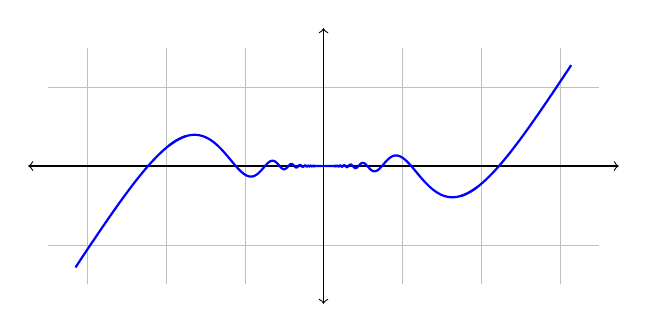
\begin{tikzpicture}
	  \draw[ultra thin,color=lightgray] (-3.5,-1.5) grid (3.5,1.5);   % coordinate grid
	  \draw[<->] (-3.75,0) -- (3.75,0);% node[right] {$x$};   % x-axis
	  \draw[<->] (0,-1.75) -- (0,1.75);% node[above] {$y$};   % y-axis
	
	%   \foreach \x/\xtext in {-4,...,-1,1,2,3,4}        % x-axis labels
	%   \draw (\x,2pt) -- (\x,-2pt) node[anchor=north, font=\footnotesize] {$\xtext$}; 
	
	%   \foreach \y/\ytext in {-4,..., -1,1,2,3, 4}           % y-axis labels
	%   \draw (2pt,\y) -- (-2pt,\y) node[anchor=east, font=\footnotesize] {$\ytext$}; 
	
	  % parametric function alpha(t)
	%   \draw [thick, samples=100,smooth] plot[variable=\t, domain=-3:3] (\t,sin(1/t));

	% \draw [thick, samples=100,smooth, color=blue] plot[variable=\t, domain=-3.5:0.935] ({\t, -1});
	% \draw [thick, samples=100,smooth, color=blue] plot[variable=\t, domain=1:3.5] ({\t, 1});

	\draw [thick, samples=100,smooth, color=blue] plot[variable=\t, domain=-0.45:-0.25] ({7*\t},{8*(\t)^2 * sin((\t)^(-1) r)});
	\draw [thick, samples=300,smooth, color=blue] plot[variable=\t, domain=-0.28:-0.004] ({7*\t},{8*(\t)^2 * sin((\t)^(-1) r)});
	\draw [thick, samples=300,smooth, color=blue] plot[variable=\t, domain=0.004:0.28] ({7*\t},{8*(\t)^2 * sin((\t)^(-1) r)});
	\draw [thick, samples=300,smooth, color=blue] plot[variable=\t, domain=-0.0045:0.0045] ({7*\t},{0});
	\draw [thick, samples=100,smooth, color=blue] plot[variable=\t, domain=0.25:0.45] ({7*\t},{8*(\t)^2 * sin((\t)^(-1) r)});
	% \draw [thick, samples=100,smooth] plot[variable=\t, domain=0.0001:3] (\t,{\t^2 * sin(1/\t)});
	% \node at (1, -1) {\color{blue} $\circ$};
	% \node at (1, 1) {\color{blue} \textbullet};
	
	\end{tikzpicture}
	\end{center}
\end{example}

There is however a limit as to how discontinuous a derivative can be. In particular the derivative of a differentiable function must have the intermediate value property.

\begin{theorem}[Darboux's Theorem]
	If $f: \R \rightarrow \R$ is differentiable then $f'$ has the intermediate value property. That is to say, if $a < b$ and $f'(a) < z < f'(b)$ then there exists $c \in (a, b)$ with $f'(c) = z$.
\end{theorem}
\begin{proof}
Given $a<b$ and $z \in \mathbb{R}$ s.t. $f^{\prime}(a)<z<f^{\prime}(b)$, we wish to show there exists $c \in(a, b)$ s.t. $f(c)=z$. We can rewrite the condition as $f^{\prime}(a)-z<0<f^{\prime}(b)-z$. Now define $g(x)=f(x)-z x,$ and note that we have $g^{\prime}(a)<0<g^{\prime}(b)$.

We want to find $c \in(a, b)$ s.t. $g^{\prime}(c)=0$. Now, $g$ is continuous (since $f$ is continuous), and thus is bounded on $[a, b]$, and the minimum is attained say at some point $k$. We can't have $k=a$, as that would imply that $g^{\prime}(a) \geq 0,$ and we also can't have $k=b$ as that would imply $g^{\prime}(b) \leq 0$. Thus $k \in(a, b),$ and we must then have $g^{\prime}(k)=0,$ and we are done.
\end{proof}

\subsection{Rolle's Theorem \& The Mean Value Theorem}

The sign of a function's derivative at a point can tell us quite a bit about the behaviour of that function near that point.
In particular, knowing that the derivative at a point vanishes can be quite useful;.

\begin{definition}[Local Maxima \& Minima]
	Let $f: \R \rightarrow \R$. If there exists $\delta$ s.t. $|x - x_0| < \delta$ implies that $f(x_0) \leq f(x)$, then we call $x$ a \vocab{local maximum}. 
	Similarly if this implies that $f(x_0) \geq f(x)$, we call $x$ a \vocab{local minimum}. 
\end{definition}

Our important result is as follows:

\begin{lemma}[Derivative of Maxima]\label{lemma:maxima}
	Let $f: \R \rightarrow \R$. If $x$ is a local maximum or minimum of $f$ and $f$ is differentiable at $x$ then $f'(x) = 0$.
\end{lemma}
\begin{proof}
	Without loss of generality, assume that $x$ is a local maximum. Then there exists $\delta$ s.t. $|h| < \delta_1$ implies that $f(x + h) \leq f(x)$. 
	
	Then if $0 < h < \delta$ we have
	$$
		\frac{f(x + h) - f(x)}{h} \geq 0,
	$$
	and thus we have $f'(x) \geq 0$.

	Similarly if $- \delta < h < 0$ we have
	$$
	\frac{f(x + h) - f(x)}{h} \leq 0,
	$$
	and thus we have $f'(x) \leq 0$. Hence $f'(x) = 0$.
\end{proof}

When we combine this result with the boundedness theorem from our discussion about continuity, we end up with \emph{Rolle's theorem}.

\begin{theorem}[Rolle's Theorem]
	Let $f: [a, b] \rightarrow \R$ be a continuous function which is differentiable on $(a, b)$. Then if $f(a) = f(b)$ then there exists $c \in (a, b)$ s.t. $f'(c) = 0$.
\end{theorem}
\begin{proof}
	Since $f$ is differentiable, it is also continuous and thus by the boundedness theorem $f$ is bounded on $[a, b]$ and these bounds are achieved.
	Thus we can let $M = \max_{x \in [a, b]} f(x)$ and $m = \min_{x \in [a, b]} f(x)$.

	If $M = m$, then $f$ must be constant and $f'(x) = 0$ for all $x \in (a, b)$, so we are done.
	Otherwise $M > f(a)$ or $m < f(a)$. If $M > f(a)$ then since the bounds are attained there exists $c \in (a, b)$ s.t. $f(c) = M$. But them $M$ is a maximum, so by our previous lemma we have $f'(c) = 0$. A similar argument works if $m < f(a)$.
\end{proof}

A direct consequence of Rolle's theorem\footnote{It's possible to establish this theorem without Rolle's theorem, and then Rolle's theorem pops out as a special case. The proof is (more or less) just what we did for Rolle's theorem laid out explicitly in the proof of this theorem.} 
is another classic theorem of analysis, the \emph{mean value theorem}, which is frequently abbreviated to MVT.

\begin{theorem}[The Mean Value Theorem]
	Let $f: [a, b] \rightarrow \R$ be a continuous function which is differentiable on $(a, b)$. Then there exists $c \in (a, b)$ s.t. $f(b) - f(a) = f'(c)(b - a)$.
\end{theorem}
\begin{proof}
	Let $k = \frac{f(a) - f(b)}{a - b}$, and define $\phi(x) = f(x) - kx$. Note that $\phi(a) = \phi(b)$. Then by Rolle's theorem there exists $c \in (a, b)$ s.t. $\phi'(c) = 0$, that is $f'(c) = k$.
\end{proof}

The mean value theorem says something notable: the size of the derivative controls the size of the function, or (in rougher terms) it puts a restriction on know `badly behaved' the function can be.
Also, if we appeal to geometric intuition (as we have tried not to, it's an easy way to go wrong) we can see that the mean value theorem says, as R. P. Burn wrote in \emph{Numbers and functions}, ``for the graph of a differentiable function, there is always a tangent parallel to the chord''. Of course, we will quickly move on from geometrical thinking.\footnote{I guess here is a good place to mention how we can reason geometrically in analysis. Drawing pictures and thinking geometrically is a great way to understand how things work, to come up with counterexamples and much more. Still it is important to remember that \emph{basically nothing in this course is provable by appealing to geometric intuition.} Instead this type of thinking should just inform the `analysis' side of us how to approach things.} 

Now let's think about applying the mean value theorem to two different functions. Suppose that $f, g : [a, b] \rightarrow \R$ is continuous and differentiable on $(a, b)$, and $g(a) \neq g(b)$. Then the mean value theorem gives us $s, t \in (a, b)$ s.t.
$$
	\frac{f(b) - f(a)}{g(b) - g(a)} = \frac{(b - a)f'(s)}{(b - a)g'(t)} = \frac{f'(s)}{g'(t)}.
$$
A stronger version of the mean value theorem says that we can take $s = t$.

\begin{theorem}[Cauchy's Mean Value Theorem]
	Let $f, g : [a, b] \rightarrow \R$ be continuous functions which are differentiable on $(a, b)$. Then there exists $c \in (a, b)$ s.t.
	$$
	(f(b) - f(a))g'(c) = f'(c)(g(b) - g(a)).
	$$
\end{theorem}
\begin{proof}
	We define the function
	\begin{align*}
		\phi(x) &= \begin{vmatrix}
			1 & 1 & 1 \\
			f(a) & f(x) & f(b) \\
			g(a) & g(x) & g(b)
			\end{vmatrix}  \\
		&= \left[f(x)g(b) - f(b)g(x)\right] - [f(a)g(b) - f(b) g(a)] + [f(a) g(x) - f(x) g(a)].
	\end{align*}
	Then $\phi$ is continuous on $[a, b]$ and differentiable on $(a, b)$\footnote{If the use of determinants bothers you, then feel free to just look at the expansion. If also remember how integrals work, you can obtain $\phi$ from working backwards from what we need to arrive at.}. Also $\phi(a) =\phi(b) = 0$. Then by Rolle's theorem, there exists $c \in (a, b)$ s.t. $\phi'(c) = 0$.
	
	Differentiating $\phi$ we then have 
	$$
	\phi'(x) = f'(x)[g(b) - g(a)] + g'(x)[f(a) - f(b)],
	$$
	and thus $\phi'(c) = 0$ gives the desired result.
\end{proof}

Cauchy's mean value theorem has many applications. For example, we can use the mean value theorem to establish L'Hôpital's rule for evaluating limits.

\begin{example}[L'Hôpitel's Rule]
	We wish to evaluate $\displaystyle \lim_{x \to 0} \frac{e^x - 1}{\sin x}$.

	By Cauchy's mean value theorem, there exist $c \in (0, x)$ s.t.
	$
	\frac{e^x - e^0}{\sin x - \sin 0} = \frac{e^c}{\cos c}.
	$
	Then $c \rightarrow 0$ as $x \rightarrow 0$, and thus we get
	$$
	\lim_{x \to 0} \frac{e^x - 1}{\sin x} = \lim_{c \to 0}\frac{e^c}{\cos c} = 1.
	$$
\end{example}

In more generality:

\begin{theorem}[L'Hôpital's Rule]
	Suppose $f, g :[a, b] \rightarrow \R$ are continuous and differentiable on $(a, b)$. Suppose that $f(a) = g(a) = 0$, that $g'(x)$ does not vanish near $a$ and $f'(x)/g'(x) \rightarrow \ell$ as $x \rightarrow a$. Then $f(x)/g(x) \rightarrow \ell$ as $x \rightarrow a$.
\end{theorem}
\begin{proof}
Since $g^{\prime}(x)$ does not vanish near $a$, we can suppose that $g^{\prime}(x) \neq 0$ for $x \in(a, b)$, as otherwise we could just consider the subinterval $\left(a, b^{\prime}\right),$ defined so that this is the case.

By Cauchy's mean value theorem we have
$$
\frac{f(x)}{g(x)}=\frac{f(x)-f(a)}{g(x)-g(a)}=\frac{f^{\prime}(c)}{g^{\prime}(c)}
$$
where $c \in(a, x)$. Then $c \rightarrow a$ as $x \rightarrow a$, and hence $f(x) / g(x) \rightarrow \ell$ as $x \rightarrow a$.
\end{proof}

The mean value theorem can also help us extend \autoref{lemma:maxima}. Knowing the sign of a derivative over some interval can tell us immediately if it is constant, increasing or decreasing.

\begin{proposition}[Sign of the Derivative]\label{prop:sign}
	Let $f: [a, b] \rightarrow \R$ be differentiable on $(a, b)$. Then the following hold.
	\begin{enumerate}[label=(\roman*)]
		\item If $f'(x) \geq 0$ for all $x \in (a, b)$, then $f$ is monotonically increasing.
		\item If $f'(x) = 0$ for all $x \in (a, b)$, then $f$ is constant.
		\item If $f'(x) \leq 0$ for all $x \in (a, b)$, then $f$ is monotonically decreasing.
	\end{enumerate}
\end{proposition}
\begin{proof}
	By the mean value theorem we have $f(x_2) - f(x_1) = (x_2 - x_1)f'(x)$ where $a < x_1 < x < x_2 < b$. Then all of the results follow by considering the sign of $f'(x)$.
\end{proof}

\subsection{Inverses of Functions}

Before we move to slightly more exciting material, there's a few things about inverses of functions that we need to get out of the way. The proofs below are straightforward but require some care (by which I mean you have to avoid messing up which letter means what).

First of all, if we know that a continuous function is strictly increasing\footnote{If a continuous function was not strictly increasing or strictly decreasing then we couldn't have a unique inverse.} then we can deduce that the function has an inverse that is continuous and strictly increasing also. A similar result holds for strictly decreasing functions.

\begin{theorem}[Continuous Inverse Theorem]
	Let $f:[a, b] \rightarrow \R$ be a continuous and strictly increasing function. Then if $c = f(a)$ and $d = f(b)$, $f:[a, b] \rightarrow [c, d]$ is bijective and the inverse $f^{-1}: [c, d] \rightarrow [a, b]$ is continuous and strictly increasing.
\end{theorem}
\begin{proof}
	As $f$ is strictly increasing, it is an injection. It is also a surjection since if $c < t < d$ then there exists $x \in (a, b)$ s.t. $f(x) = t$. Thus $f$ is a bijection, and has an inverse $f^{-1}$.

	Since $f$ is strictly increasing, we can write this as $x_1 < x_2 \iff f(x_1) < f(x_2)$, so letting $f(x_1) = y_1$ and $f(x_2) = y_2$ we have 
	$f^{-1}(y_1) < f^{-1}(y_2) \iff y_1 < y_2$. Thus $f^{-1}$ is also strictly increasing.
	
	Now we will show $f^{-1}$ is continuous at some $y \in [c, d]$.
	Given $\varepsilon > 0$, 
	let $x = f^{-1}(y)$. If $x \neq a, b$, we can find $\delta$ s.t.
	$$
		f(x - \varepsilon) \leq f(x) - \delta < f(x) < f(x) + \delta \leq f(x + \varepsilon).
	$$
	But then $|z - y| < \delta$ implies that $x - \varepsilon < f^{-1}(z) < x + \varepsilon$, so $|f^{-1}(z) - f^{-1}(y)| < \varepsilon$.
	Thus $f^{-1}$ is continuous on $(a, b)$

	Otherwise, if $x = a$ we have $f(x) < f(x + \varepsilon)$. Then $|z - y| < f(x + \varepsilon) - f(x)$ implies that $|f^{-1}(z) - f^{-1}(y)| < \varepsilon$, so $f^{-1}$ is continuous at $c$. A similar argument shows that it is continuous at $d$.
\end{proof}

Now this \emph{is} the differentiability section, so we can also describe what the derivative of a differentiable function's inverse is. This result is known as the one variable \emph{inverse function theorem}.

\begin{theorem}[Inverse Function Theorem]
	Let $f:[a, b] \rightarrow \R$ be continuous, strictly increasing, and differentiable on $(a, b)$.
	Then let $f(a) = c$ and $f(b) = d$. Then $f:[a, b] \rightarrow [c, d]$ is a bijection, and $f^{-1}$ is differentiable on $(c, d)$, with
	$$
	(f^{-1})'(x) = \frac{1}{f'(f^{-1}(x))}.
	$$
\end{theorem}
\begin{proof}
	By our previous theorem, $f$ is a bijection and $f^{-1}$ is a continuous and strictly increasing function. Let $y = f(x)$, with $x \in (a, b)$. We wish to show that $g'(y) = 1/f'(x)$.

	Given $k \neq 0$, let $h$ be given by $y + k = f(x + h)$, that is, $f^{-1}(y + k) = x + h$, where $h \neq 0$. Then
	$$
	\frac{f^{-1}(y + k) - f^{-1}(y)}{k} = \frac{h}{f(x + h) - f(x)}.
	$$
	Then since $f'(x) > 0$ and $f^{-1}$ is continuous (so $h \rightarrow 0$ as $k \rightarrow 0$) we have $k \to 0$ 
	$$
	\lim_{k \to 0} \frac{f^{-1}(y + k) - f^{-1}(y)}{k} = \lim_{h \to 0} \frac{x + h - x}{f(x + h) - f(x)} = \frac{1}{f'(x)},
	$$
	as required.
\end{proof}

\subsection{Taylor's Theorem}

We are now going to think about functions where we can take derivatives a number of times (getting higher-order derivatives).
We will begin by looking at how we can get an analogue of Rolle's theorem for higher-order derivatives. I will apologise in advance that this discussion is a bit long, so feel free to just skip to Taylor's theorem.

The following generalisation will come directly from Rolle's theorem.
\begin{theorem}[Higher-Order Rolle's Theorem]
	Let $f$ be continuous and $n-1$-times differentiable on $[a, b]$ and also $n$-times differentiable on $(a, b)$. Then if $f(a) = f'(a) = f''(a) = \cdots = f^{(n - 1)}(a) = 0$ and $f(b) = 0$ then there is a $c \in (a, b)$ s.t. $f^{(n)}(c) = 0$.
\end{theorem}
\begin{proof}
	Since $f(a) = f(b)$, by Rolle's theorem there exists $c_1 \in (a, b)$ s.t. $f'(c_1) = 0$. Then since $f'(a) = f'(c_1) = 0$, we can use Rolle's theorem again to obtain $c_2 \in (a, c_1)$ s.t. $f''(c_2) = 0$. Continuing on like this we obtain a $c_{n} \in (a, b)$ s.t. $f^{(n)}(c_n) = 0$, as required.
\end{proof}

We can also attempt to get some sort of `higher-order' mean value theorem. Recall that our proof of the mean value theorem was more or less as follows:
\begin{quotation}\noindent
	\emph{Define the function $\phi(x) = f(x) - kx$, where we choose $k$ s.t. the conditions of Rolle's theorem are satisfied.
	Then apply Rolle's theorem to $\phi$.}
\end{quotation}
We can try and do the same with a more elaborate construction. We will do this in three steps.
\begin{enumerate}
	\item Construct a polynomial $P(x)$ s.t. $P(a) = f(a)$, $P'(a) = f'(a)$, and so on until $P^{(n - 1)}(a) = f^{(n - 1)}(a)$.
	\item Construct another polynomial\footnote{We can think of this as the `error correcting term', because it fixes the discrepancy between $f(b)$ and $P(b)$ while not ruining the previous construction.} $E(x)$ s.t. $E^{(r)}(a) = 0$ for $r = 0, 1, \dots, n - 1$, but with $E(b) = f(b) - P(b)$.
	\item Take $\phi(x) = f(x) - P(x) - E(x)$.
\end{enumerate}
If we construct $\phi(x)$ in this way, then we will have $\phi(a) = \phi'(a) = \cdots = \phi^{(n - 1)}(a) = 0$, and also $\phi(b) = 0$, so it will satisfy our higher-order Rolle's theorem.

\begin{aside}{Aside: Constructing Our Polynomials}

	While it is likely you have seen a construction for $P$ before, I'd like to take a minute to spell it out in detail because it has some nice ideas.

	To construct this polynomial, what we really need is some construction of a term which affects the value of the polynomial at a point $a$ if and only if we are considering a certain derivative. We can do this as follows:
	$$
		Q_{k}(x) = \frac{(x - a)^k}{k!}.
	$$
	We can then (by taking derivatives) find that the value of this term is
	$$
	Q_k^{(j)}(a) = \begin{cases}
        1 &\mbox{if } j = k, \\
        0 &\mbox{if } j \neq k
       \end{cases}
	$$
	With this we can immediately write down an explicit construction for $P(x)$.
	\begin{align*}
		P(x) &= \sum_{k = 0}^{n - 1} f^{(k)}(a) Q_k(x) = \sum_{k = 0}^{n - 1} \frac{f^{(k)}(a)}{k!}(x - a)^k \\
		&= f(a) + f'(a) (x - a) + \frac{f''(a)}{2} (x - a)^2 + \cdots + \frac{f^{(n - 1)(a)}}{(n - 1)!} (x - a)^{n - 1}.
	\end{align*}

	This polynomial is known as the \vocab{Taylor polynomial} of degree $n - 1$ for $f$ about $a$. 

	We can use the exact same method to construct $E(x)$. 
	We need to not affect the first $n - 1$ derivatives at $x = a$, so we will need to add some multiple of $Q_{n}(x)$. However, this time we care about the value of the undifferentiated term at $x = b$:
	$$
	Q_{n}(b) = \frac{(b - a)^n}{n!}.
	$$
	Since we want $E(b) = f(b) - P(b)$, if we are going to have $E(x) = \lambda Q_n(x)$ we are going to need
	\begin{align*}
		\lambda Q_{n}(b) &= \lambda \frac{(b - a)^n}{n!} = f(b) - P(b) \\
\implies \lambda &= \frac{[f(b) - P(b)] \cdot n!}{(b - a)^n}.
	\end{align*}
	And thus we get
	\begin{align*}
		E(x) &= \frac{[f(b) - P(b)] \cdot n!}{(b - a)^n} Q_n(x) \\
		&= \left[f(b) - P(b)\right]\left(\frac{x - a}{b - a}\right)^n.
	\end{align*}
\end{aside}

Now with the constructions as above, we can write down $\phi(x) = f(x) - P(x) - E(x)$.
Then since $\phi(x)$ satisfies all of the conditions of our higher-order Rolle's theorem, there exists $c \in (a, b)$ s.t. $\phi^{(n)}(c) = 0$. 

Taking the $n$th derivative, since $P$ is a degree $n - 1$ polynomial and thus has a zero derivative, we get
\begin{align*}
	\phi^{(n)}(c) &= f^{(n)}(c) - [f(b) - P(b)] \cdot \frac{n!}{(b - a)^n} = 0 \\
\implies f(b)  &= P(b) + \frac{f^{(n)}(c)}{n!}(b - a)^n.
\end{align*}
for some $c \in (a, b)$. 

This result is Taylor's theorem, specially Taylor's theorem with the Lagrange form of the remainder. For completeness, this proof is given in a standalone form below.

\begin{theorem}[Taylor's Theorem with Lagrange Remainder]
	Let $f$ be continuous and $(n - 1)-$times differentiable on $[a, b]$ and $n$-times differentiable on $(a, b)$. Then we have
	$$
	f(b) = f(a) + f'(a)(b - a) + \cdots + \frac{f^{(n - 1)}(a)}{(n - 1)!}(b - a)^{n - 1} + \frac{f^{(n)}(c)}{n!}(b - a)^n,
	$$
	for some $c \in (a, b)$.
\end{theorem}
\begin{proof}
	We define
	$$
	\phi(x) = f(x) - \sum_{k = 0}^{n - 1} \frac{f^{(k)}(a)}{k!}(x - a)^k - M \left(\frac{x - a}{b - a}\right)^n,
	$$
	where $M$ is chosen s.t. $\phi(a) = \phi(b) = 0$.
	Then differentiating we have $\phi(a) = \phi'(a) = \cdots = \phi^{(n - 1)}(a) = 0$. 

	Then since $\phi(a) = \phi(b)$, there exists $c_1 \in (a, b)$ s.t. $\phi'(c_1) = 0$. Similarity $\phi'(a) = \phi'(c_1) = 0$, and thus there exists $c_2 \in (a, c_1)$ s.t. $\phi''(c_2) = 0$. Continuing on in this way, we find a $c_{n}$ s.t. $\phi^{(n)}(c_n) = 0$, where $c_n \in (a, b)$. 

	Then differentiating again we have
	$$
	\phi^{(n)}(c) = f^{(n)}(c) - \frac{M \cdot n!}{(b - a)^n} = 0.
	$$
	Now we know that $M$ is s.t. $\phi(b) = 0$, so we get
	$$
	M = f(b) - \sum_{k = 0}^{n - 1}\frac{f^{(k)}(a)}{k!} (b - a)^n.
	$$
	Thus we have
	\begin{align*}
		f^{(n)}(c) &= \frac{M \cdot n!}{(b - a)^n} = \left(f(b) - \sum_{k = 0}^{n - 1}\frac{f^{(k)}(a)}{k!} (b - a)^n\right) \cdot \frac{n!}{(b - a)^n} \\
\implies f(b) &= f(a) + f'(a)(b - a) + \cdots + \frac{f^{(n - 1)}(a)}{(n - 1)!}(b - a)^{n - 1} + \frac{f^{(n)}(c)}{n!}(b - a)^n,
	\end{align*}
	where $c \in (a, b)$ as required.
\end{proof}


So we have Taylor's theorem (which in this case can be thought of as a higher-order mean value theorem), let's try and do something with it. One of the main uses of Taylor's theorem is in giving us an infinite series which converges to the value of our function. This involves considering the terms of the degree $n$ taylor polynomial for increasing values of $n$, as we shall see.

Doing this type of problem has two main steps.
\begin{enumerate}
	\item Write down Taylor's theorem for the case of the function being considered.
	\item Show that the error term tends to zero as $n$ goes to infinity.
\end{enumerate}
We see how this is done using a Tripos question from 2010 (so eh spoilers I guess).

\begin{example}[Using Taylor's Theorem -- Part IA, 2010 Paper 1, Q10]
\emph{Problem}. Suppose that $e: \mathbb{R} \rightarrow \mathbb{R}$ is a differentiable function s.t. $e(0)=1$ and $e^{\prime}(x)=e(x)$ for all $x \in \mathbb{R}$. Use Taylor's theorem with the remainder in Lagrange's form to prove that
$$
e(x)=\sum_{n \geqslant 0} \frac{x^{n}}{n !} \quad \text { for all } \quad x \in \mathbb{R}
$$
[No property of the exponential function may be assumed.]

\emph{Solution}. We begin by noting that $e(x)$ is infinitely differentiable, with $e^{(n)}(x) = e(x)$. Indeed this is true for $n = 1$, and then it follows by induction for all $n$. Thus Taylor's theorem with Lagrange Remainder holds for all $n \in \N$.

Thus for all $n \in \N$ we have (using $e^{(n)}(0) = 1$ and $e^{(n)}(c) = e(c)$)
$$
e(x) = \sum_{k = 0}^{n - 1}\frac{x^k}{k!} + \frac{e(c) x^n}{n!} 
$$
for some $c \in (0, x)$.
And thus it suffices to show that $\frac{e(c)x^n}{n!} \rightarrow 0$ as $n \rightarrow \infty$, since that would imply that $e(x) - \sum_{k = 0}^{n - 1} \frac{x^k}{k!} \rightarrow 0$ as $n \rightarrow \infty$.
Now $e(t)$ is differentiable and hence continuous on $[0, x]$, and thus is bounded. So it suffices to show that $x^n/n! \rightarrow 0$, which holds.

Thus
$$
e(x) = \sum_{n = 0}^{\infty} \frac{x^n}{n!},
$$
as required.
\end{example}


Now it is \emph{not} the case that the remainder term always goes to zero. A common counterexample is $f(x) = \exp(-1/x^2)$ for $x \neq 0$ with $f(0) = 0$.

\clearpage